\documentclass[11pt,a4paper]{article}

% ---------------------------------------------------------------------------
% Packages
% ---------------------------------------------------------------------------
\usepackage[a4paper,margin=1in]{geometry}
\usepackage[utf8]{inputenc}
\usepackage[T1]{fontenc}
\usepackage{lmodern}
\usepackage{graphicx}
\usepackage{tikz}
\usetikzlibrary{arrows.meta,positioning,shapes.geometric,fit,backgrounds,calc,shadows}
\usepackage{booktabs}
\usepackage{array}
\usepackage{hyperref}
\usepackage{enumitem}
\usepackage{xcolor}
\usepackage{caption}
\usepackage{amsmath}
\usepackage{titlesec}
\usepackage{fancyhdr}
\usepackage{tabularx}
\usepackage{float}
\usepackage{xurl}

% Ragged-right table columns: justified text in narrow columns leaves wide gaps.
\newcolumntype{L}[1]{>{\raggedright\arraybackslash}p{#1}}
\newcolumntype{Y}{>{\raggedright\arraybackslash}X}

\hypersetup{
    colorlinks=true,
    linkcolor=blue!50!black,
    citecolor=blue!50!black,
    urlcolor=blue!50!black,
    pdftitle={DiagramForge: A Cloud-Native DevSecOps Platform for AI-Assisted Diagram Generation}
}

\pagestyle{fancy}
\fancyhf{}
\fancyhead[L]{\small DiagramForge --- Architecture \& Implementation Report}
\fancyhead[R]{\small \thepage}
\renewcommand{\headrulewidth}{0.3pt}

\titleformat{\section}{\normalfont\Large\bfseries}{\thesection}{1em}{}
\titleformat{\subsection}{\normalfont\large\bfseries}{\thesubsection}{1em}{}

% Lets long \texttt{} identifiers wrap instead of running into the margin.
\emergencystretch=3em

% ---------------------------------------------------------------------------
% Diagram palette and styles (shared by every figure)
% ---------------------------------------------------------------------------
\definecolor{clientTier}{RGB}{204,229,255}   % client / browser
\definecolor{appTier}{RGB}{212,237,218}      % application workloads
\definecolor{dataTier}{RGB}{255,229,204}     % data stores
\definecolor{ciTier}{RGB}{255,210,210}       % CI/CD and failure outcomes
\definecolor{infraTier}{RGB}{232,232,232}    % infrastructure
\definecolor{secGate}{RGB}{255,242,204}      % decision / security gates
\definecolor{extTier}{RGB}{230,230,250}      % third-party services

\tikzset{
    every node/.append style={align=center},
    box/.style={rectangle,draw=black,thick,rounded corners=2pt,minimum height=0.9cm,
        minimum width=2.6cm,font=\small,drop shadow={opacity=0.25}},
    gate/.style={diamond,draw=black,thick,aspect=2.4,font=\scriptsize,
        fill=secGate,inner sep=1pt},
    boundary/.style={rectangle,draw=black!70,dashed,thick,rounded corners=4pt},
    arr/.style={-{Latex[length=2.6mm,width=1.9mm]},thick},
    darr/.style={-{Latex[length=2.6mm,width=1.9mm]},thick,dashed},
    lbl/.style={font=\scriptsize,fill=white,inner sep=1.2pt},
    uc/.style={rectangle,rounded corners=8pt,draw,thick,minimum width=2.8cm,
        minimum height=0.62cm,font=\scriptsize},
    actor/.style={ellipse,draw,thick,minimum width=2.1cm,minimum height=0.9cm,font=\small}
}

\newcommand{\reqid}[1]{\texttt{#1}}

% ---------------------------------------------------------------------------
\definecolor{amritaMaroon}{HTML}{A4163F}
\hypersetup{
    pdftitle={DiagramForge: A Cloud-Native DevSecOps Platform for AI-Assisted Diagram Generation},
    pdfauthor={Mahakisore M, Yashwanth B (Team D11)}
}

\begin{document}

% ------------------------------- Title page --------------------------------
\begin{titlepage}
    \centering
    
\includegraphics[width=0.78\textwidth]{figures/amrita-logo.png}\\[0.4cm]
    {\large School of Artificial Intelligence}\\[0.1cm]
    {\normalsize Amrita Vishwa Vidyapeetham, Ettimadai, Coimbatore}\\[1.2cm]

    {\large\bfseries 22AIE305 --- Introduction to Cloud Computing}\\[0.2cm]
    {\normalsize Course Project Report}\\[1.0cm]

    {\color{amritaMaroon}\rule{\textwidth}{1.2pt}}\\[0.5cm]
    {\LARGE\bfseries DiagramForge}\\[0.35cm]
    {\large A Cloud-Native DevSecOps Platform for\\ AI-Assisted Diagram Generation}\\[0.3cm]
    {\normalsize\itshape Architecture, Implementation, and CI/CD Pipeline Report}\\[0.3cm]
    {\color{amritaMaroon}\rule{\textwidth}{1.2pt}}\\[1.2cm]

    {\large\bfseries Team D11}\\[0.4cm]
    \begin{tabular}{ll}
        \toprule
        \textbf{Name} & \textbf{Roll Number} \\
        \midrule
        Mahakisore M & CB.SC.U4AIE24333 \\
        Yashwanth B  & CB.SC.U4AIE24360 \\
        \bottomrule
    \end{tabular}\\[1.2cm]

    {\normalsize Under the guidance of}\\[0.15cm]
    {\large\bfseries Dr.\ Keerthika}\\

    \vfill
    {\normalsize \today}
\end{titlepage}

\begin{abstract}
\noindent
DiagramForge (repository name \texttt{Diagram-Ops}) is a cloud-native learning
platform built around a deliberately small application: a user describes a
system in natural language, a large language model (LLM) converts that
description into Mermaid diagram syntax, and the browser renders it. The
application is intentionally minimal so that the engineering effort can
concentrate on the platform that surrounds it --- containerisation,
infrastructure as code, Kubernetes orchestration, a security-gated CI/CD
pipeline, and (in later phases) observability, progressive delivery, and
disaster recovery. This report documents the system as an industry-style
architecture and implementation record: functional and non-functional
requirements; the application's internal design (context, use case,
component, data, control-flow, and state views); the infrastructure
topology on AWS; and, in particular detail, the Jenkins-based DevSecOps
pipeline that gates every change behind static analysis (SonarQube),
software-composition analysis (OWASP Dependency-Check), and container image
scanning (Trivy) before an image may reach the container registry. Real
defects found while hardening that pipeline are documented as case studies,
including a false-positive CVE caused by an NVD CPE vendor/product collision
between the MongoDB server and its Node.js driver, and a class of image
vulnerabilities caused by an unused \texttt{npm} CLI left in the runtime
container.
\end{abstract}

\tableofcontents
\listoffigures
\newpage

% =============================================================================
\section{Introduction}
% =============================================================================

\subsection{Motivation}
Most student DevOps projects struggle for one of two opposite reasons:
the application is either too trivial to justify a real platform, or too
complex to finish. DiagramForge resolves this tension deliberately by
keeping the \emph{application} small --- three persisted entities (users,
diagrams, provider usage) and a single LLM-backed generation endpoint ---
while growing the \emph{platform} around it, phase by phase, until its
operational practices resemble what a small production team would actually
run: infrastructure as code, a security-gated pipeline, GitOps delivery,
observability, and explicit cost discipline.

\subsection{Objectives}
\begin{itemize}[nosep]
    \item Build a working three-tier application (React, Express, MongoDB)
        with real authentication, real LLM integration, and automated tests.
    \item Provision every piece of cloud infrastructure through Terraform,
        never through manual console operations.
    \item Enforce a non-negotiable quality bar before any container image
        reaches the registry: static analysis, dependency vulnerability
        scanning, and image vulnerability scanning, each able to fail the
        build independently.
    \item Run the application on Kubernetes (Amazon EKS), delivered through
        GitOps rather than direct \texttt{kubectl} access by a human.
    \item Treat cost as a first-class constraint --- every phase's monthly
        cost is known and budgeted in advance.
\end{itemize}

\subsection{Scope and Guiding Principle}
The project's own guiding principle is deliberately blunt: \emph{``Keep the
app simple. Make the platform serious.''} This report follows the same
split. Section~\ref{sec:app-design} covers the application's internal
design; Section~\ref{sec:devsecops} covers the platform, which is the
actual subject of the project.

% =============================================================================
\section{Requirements Engineering}
% =============================================================================

\subsection{Actors}
\begin{table}[H]
\centering
\begin{tabularx}{\textwidth}{@{}l Y@{}}
\toprule
\textbf{Actor} & \textbf{Description} \\
\midrule
Guest & An unauthenticated visitor who may register or log in. \\
Registered User & An authenticated user who generates, saves, edits, and
    exports diagrams. \\
LLM Provider (system) & Groq (primary) or Anthropic Claude (fallback);
    external systems the backend calls to convert text to Mermaid syntax. \\
Scheduler (system) & Triggers scheduled operational jobs such as nightly
    database backups. \\
Operator / SRE & Interacts with the platform only through Git commits and
    monitoring dashboards --- never directly with the running application. \\
\bottomrule
\end{tabularx}
\caption{System actors}
\end{table}

\subsection{Functional Requirements}
The full specification enumerates requirements as \reqid{FR-<area><n>},
prioritised with RFC~2119 keywords (\textbf{MUST}, \textbf{SHOULD},
\textbf{MAY}). Table~\ref{tab:fr-summary} summarises each area and calls
out the individual requirements that most directly shaped the design in
Section~\ref{sec:app-design}.

\begin{table}[H]
\centering
\begin{tabularx}{\textwidth}{@{}L{3.3cm} c Y@{}}
\toprule
\textbf{Area} & \textbf{Count} & \textbf{Architecturally significant requirements} \\
\midrule
Authentication \newline (\reqid{FR-A*}) & 9 &
    Registration and login with bcrypt password hashing (cost $\geq$ 12);
    JWT-protected routes return \texttt{401} when the token is missing,
    invalid, or expired. \\
Generation \newline (\reqid{FR-G*}) & 9 &
    \reqid{FR-G4}: on a syntax/type mismatch, retry \emph{once}, using the
    \emph{same} provider that responded (a ``sticky retry'') --- a
    formatting glitch never escalates to the paid provider.
    \reqid{FR-G5}: automatic failover to the secondary provider.
    \reqid{FR-G6}: a hard daily call cap on the paid provider, enforced
    \emph{before} the call. \reqid{FR-G7}: generation never persists
    anything; the user must explicitly save. \\
Diagram management \newline (\reqid{FR-D*}) & 8 &
    \reqid{FR-D7}: a user may only read, update, or delete their own
    diagrams; any attempt on another user's diagram returns \texttt{404}
    rather than \texttt{403}, so the response never confirms that the
    resource exists. \\
Export \newline (\reqid{FR-E*}) & 3 &
    SVG download, PNG download, copy raw Mermaid source. \\
Operational \newline (\reqid{FR-O*}) & 6 &
    \reqid{FR-O1}/\reqid{FR-O2}: separate liveness (\texttt{/healthz}) and
    readiness (\texttt{/readyz}) probes, so a transient database blip
    cannot make Kubernetes restart every pod at once.
    \reqid{FR-O6}: graceful shutdown on \texttt{SIGTERM}. \\
\bottomrule
\end{tabularx}
\caption{Functional requirement areas}
\label{tab:fr-summary}
\end{table}

\subsection{Non-Functional Requirements}
\begin{table}[H]
\centering
\begin{tabularx}{\textwidth}{@{}L{2.9cm} Y L{4.2cm}@{}}
\toprule
\textbf{Category} & \textbf{Key requirement} & \textbf{Verification} \\
\midrule
Performance \newline (\reqid{NFR-P*}) &
    95\% of generations complete within 10\,s; 95\% of non-LLM requests
    within 300\,ms. &
    Prometheus latency histograms (Phase~9). \\
Availability \newline (\reqid{NFR-A*}) &
    99\% non-5xx SLO over a rolling 7 days; RTO $\leq$ 45\,min,
    RPO $\leq$ 24\,h. &
    Recording rules, burn-rate alerts, timed restore drills. \\
Security \newline (\reqid{NFR-S*}) &
    No secret in Git, image layers, or logs; non-root containers.
    \textbf{A build fails on any dependency with CVSS $\geq$ 8, or any
    fixable HIGH/CRITICAL image vulnerability} (\reqid{NFR-S5}). &
    OWASP Dependency-Check and Trivy gates (Phase~6 --- this report's
    primary subject). \\
Scalability \newline (\reqid{NFR-SC*}) &
    Backend scales from 3 to 10 pods above 70\% average CPU; stateless
    backend. &
    HPA plus load test. \\
Observability \newline (\reqid{NFR-O*}) &
    Per-route rate, errors, and latency visible; logs survive restarts and
    are queryable by request ID. &
    Grafana, Loki (Phases~9, 15). \\
Cost \newline (\reqid{NFR-C*}) &
    Total AWS spend under \$40/month with disciplined teardown. &
    AWS Budget alert at 60\%. \\
\bottomrule
\end{tabularx}
\caption{Non-functional requirement categories}
\label{tab:nfr-summary}
\end{table}

% =============================================================================
\section{System Architecture}
\label{sec:architecture}
% =============================================================================

\subsection{System Context}
Figure~\ref{fig:context} places the system in its operating environment.
The Operator never touches the running application directly: they interact
only through Git, which drives the pipeline, and through dashboards, which
are read-only. This separation is the architectural point of GitOps --- the
cluster's desired state lives in a repository, not in anyone's memory of
commands they once ran against it. The dashed edge to the Anthropic API is
the failover path; it is exercised rarely by design, which is exactly why
it has a dedicated automated test.

\begin{figure}[H]
\centering
\resizebox{\textwidth}{!}{%
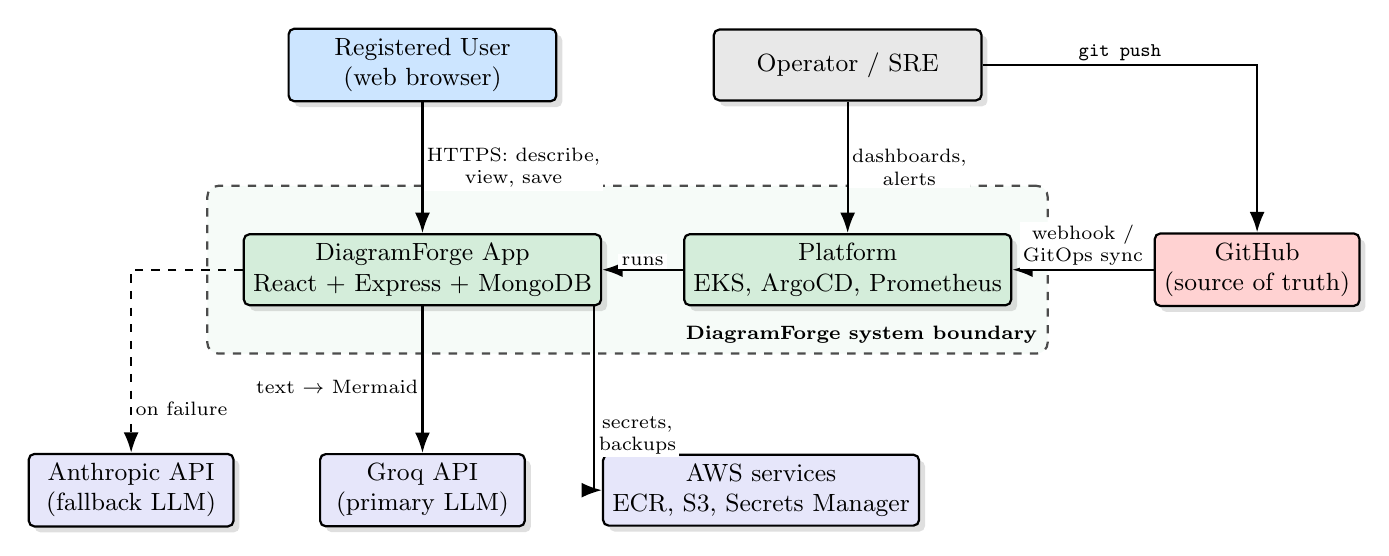
\begin{tikzpicture}
    % actors
    \node[box,fill=clientTier,minimum width=3.4cm] (user)     at (-2.7, 0)   {Registered User\\(web browser)};
    \node[box,fill=infraTier,minimum width=3.4cm]  (operator) at ( 2.7, 0)   {Operator / SRE};
    % system
    \node[box,fill=appTier,minimum width=4.1cm]    (app)      at (-2.7,-2.6) {DiagramForge App\\React + Express + MongoDB};
    \node[box,fill=appTier,minimum width=4.1cm]    (platform) at ( 2.7,-2.6) {Platform\\EKS, ArgoCD, Prometheus};
    % external systems
    \node[box,fill=ciTier]                          (github)   at ( 7.9,-2.6) {GitHub\\(source of truth)};
    \node[box,fill=extTier]                         (claude)   at (-6.4,-5.4) {Anthropic API\\(fallback LLM)};
    \node[box,fill=extTier]                         (groq)     at (-2.7,-5.4) {Groq API\\(primary LLM)};
    \node[box,fill=extTier,minimum width=3.4cm]     (aws)      at ( 1.6,-5.4) {AWS services\\ECR, S3, Secrets Manager};

    \begin{scope}[on background layer]
        \node[boundary,fill=appTier!20,fit=(app)(platform),inner xsep=0.45cm,inner ysep=0.6cm,
            label={[anchor=south east,font=\bfseries\scriptsize,inner sep=4pt]south east:DiagramForge system boundary}] {};
    \end{scope}

    \draw[arr]  (user) -- node[lbl,right]{HTTPS: describe,\\view, save} (app);
    \draw[arr]  (operator) -- node[lbl,right]{dashboards,\\alerts} (platform);
    \draw[arr]  (operator.east) -| node[lbl,pos=0.25,above]{\texttt{git push}} (github.north);
    \draw[arr]  (github.west) -- node[lbl,above]{webhook /\\GitOps sync} (platform.east);
    \draw[arr]  (platform.west) -- node[lbl,above]{runs} (app.east);
    \draw[arr]  (app.south) -- node[lbl,pos=0.55,left]{text $\to$ Mermaid} (groq.north);
    \draw[darr] (app.west) -| node[lbl,pos=0.88,right]{on failure} (claude.north);
    \draw[arr]  ($(app.south east)+(-0.1,0)$) |- node[lbl,pos=0.35,right]{secrets,\\backups} (aws.west);
\end{tikzpicture}}
\caption{System context diagram}
\label{fig:context}
\end{figure}

\subsection{High-Level Runtime Architecture}
Figure~\ref{fig:highlevel} shows the target runtime topology on Amazon EKS.
The cluster itself is provisioned and verified (Phase~4); the application
workloads are deployed onto it through Helm and ArgoCD in Phases~7--8, and
today the same three-tier stack runs locally under Docker Compose. The
frontend pod runs nginx, which serves the built React bundle and
reverse-proxies \texttt{/api/*} to the backend service. The frontend calls
\texttt{/api/\ldots} as a \emph{relative} path, so the browser only ever
talks to a single origin: no CORS configuration is needed, and no API URL is
baked into the bundle. This matters because Vite resolves environment
variables at \emph{build} time, not run time --- a baked-in absolute URL
would tie one image to one environment, which is the most common way this
class of architecture breaks.

\begin{figure}[H]
\centering
\resizebox{\textwidth}{!}{%
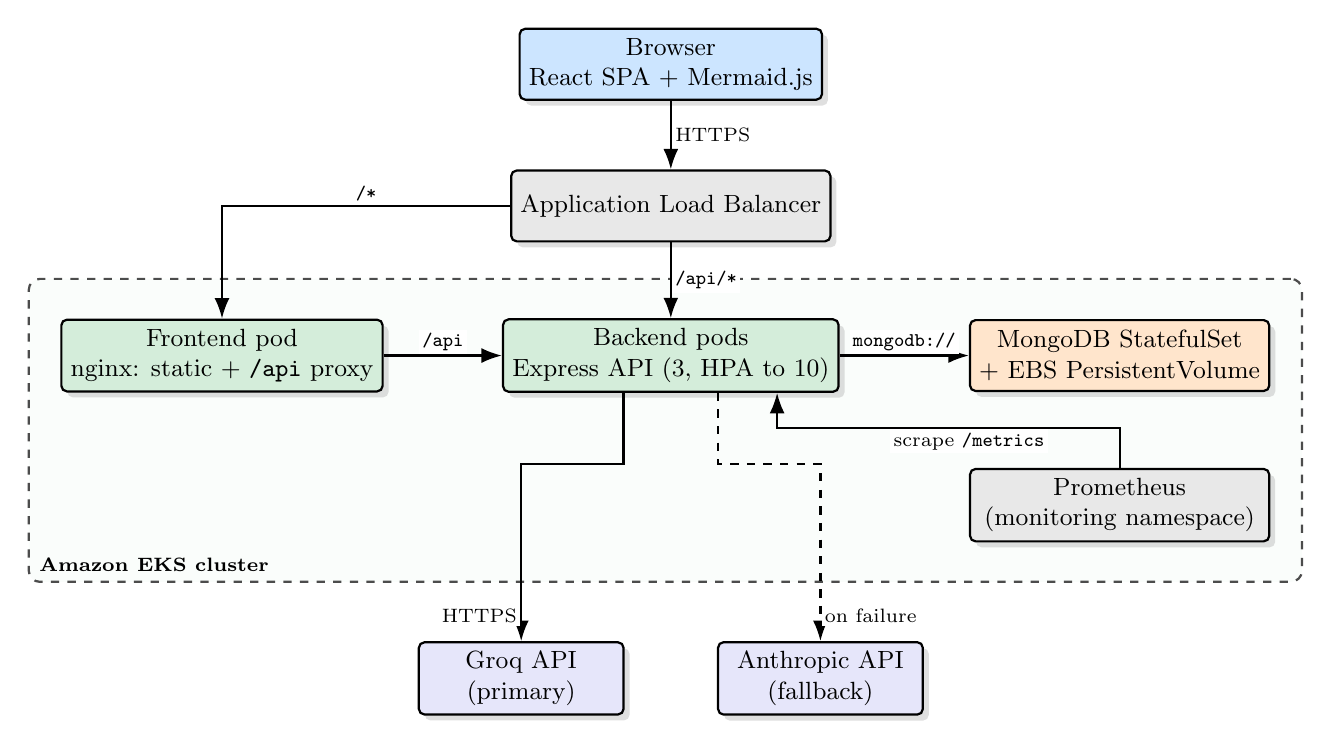
\begin{tikzpicture}
    \node[box,fill=clientTier,minimum width=3.4cm] (browser) at ( 0, 0)   {Browser\\React SPA + Mermaid.js};
    \node[box,fill=infraTier,minimum width=3.4cm]  (alb)     at ( 0,-1.8) {Application Load Balancer};
    \node[box,fill=appTier,minimum width=3.8cm]    (fe)      at (-5.7,-3.7) {Frontend pod\\nginx: static + \texttt{/api} proxy};
    \node[box,fill=appTier,minimum width=3.9cm]    (be)      at ( 0,-3.7) {Backend pods\\Express API (3, HPA to 10)};
    \node[box,fill=dataTier,minimum width=3.8cm]   (mongo)   at ( 5.7,-3.7) {MongoDB StatefulSet\\+ EBS PersistentVolume};
    \node[box,fill=infraTier,minimum width=3.8cm]  (prom)    at ( 5.7,-5.6) {Prometheus\\(monitoring namespace)};
    \node[box,fill=extTier]                         (groq)    at (-1.9,-7.8) {Groq API\\(primary)};
    \node[box,fill=extTier]                         (claude)  at ( 1.9,-7.8) {Anthropic API\\(fallback)};

    \begin{scope}[on background layer]
        \node[boundary,fill=appTier!12,fit=(fe)(be)(mongo)(prom),inner xsep=0.4cm,inner ysep=0.5cm,
            label={[anchor=south west,font=\bfseries\scriptsize,inner sep=4pt]south west:Amazon EKS cluster}] {};
    \end{scope}

    \draw[arr]  (browser) -- node[lbl,right]{HTTPS} (alb);
    \draw[arr]  (alb.west) -| node[lbl,pos=0.25,above]{\texttt{/*}} (fe.north);
    \draw[arr]  (alb) -- node[lbl,right]{\texttt{/api/*}} (be);
    \draw[arr]  (fe) -- node[lbl,above]{\texttt{/api}} (be);
    \draw[arr]  (be) -- node[lbl,above]{\texttt{mongodb://}} (mongo);
    \draw[arr]  ($(be.south)+(-0.6,0)$) -- ++(0,-0.9) -| node[lbl,pos=0.93,left]{HTTPS} (groq.north);
    \draw[darr] ($(be.south)+( 0.6,0)$) -- ++(0,-0.9) -| node[lbl,pos=0.93,right]{on failure} (claude.north);
    \draw[arr]  (prom.north) |- node[lbl,pos=0.72,below]{scrape \texttt{/metrics}} ($(be.south)+(1.35,-0.45)$) -- ($(be.south)+(1.35,0)$);
\end{tikzpicture}}
\caption{High-level runtime architecture on Amazon EKS}
\label{fig:highlevel}
\end{figure}

\subsection{Layered Backend Component Architecture}
The backend follows a strict layering discipline (Figure~\ref{fig:layers}):
controllers are thin and never touch models directly, all business logic
lives in services, and the choice of LLM provider is hidden behind an
interface. \texttt{ILLMProvider} is the architecturally important
abstraction --- \texttt{ProviderRegistry} depends on the \emph{interface},
never on \texttt{GroqProvider} or \texttt{ClaudeProvider} directly
(Dependency Inversion). That buys three concrete properties: adding a third
provider is one new class and no other change; the whole test suite runs
against a mocked interface with zero API calls and zero cost; and swapping
which provider is primary is a single environment variable.

\begin{figure}[H]
\centering
\begin{tikzpicture}[node distance=0.55cm and 1.6cm]
    \node[box,fill=clientTier,minimum width=9cm] (mw)   {HTTP middleware\\auth $\cdot$ rate limit $\cdot$ metrics $\cdot$ structured logging};
    \node[box,fill=appTier,below=of mw,minimum width=9cm] (ctrl) {Controllers\\\texttt{AuthController} $\cdot$ \texttt{DiagramController}};
    \node[box,fill=appTier,below=of ctrl,minimum width=9cm] (svc) {Services\\\texttt{AuthService} $\cdot$ \texttt{DiagramService} $\cdot$ \texttt{CostGuard}};

    \node[box,fill=secGate,below=0.7cm of svc,xshift=-2.6cm,minimum width=4.4cm] (registry) {\texttt{ProviderRegistry}};
    \node[box,fill=infraTier,below=0.7cm of registry,minimum width=4.4cm] (iface) {\texttt{«interface»}\\\texttt{ILLMProvider}};
    \node[box,fill=extTier,below=0.6cm of iface,xshift=-1.35cm,minimum width=2.1cm] (groq) {\texttt{GroqProvider}};
    \node[box,fill=extTier,right=0.35cm of groq,minimum width=2.1cm] (claude) {\texttt{ClaudeProvider}};

    \node[box,fill=dataTier,below=0.7cm of svc,xshift=2.9cm,minimum width=3.4cm] (models) {Mongoose models\\\texttt{User} $\cdot$ \texttt{Diagram} $\cdot$ \texttt{ProviderUsage}};
    \node[box,fill=dataTier,below=0.9cm of models,minimum width=3.4cm] (mongo) {MongoDB};

    \draw[arr] (mw) -- (ctrl);
    \draw[arr] (ctrl) -- (svc);
    \draw[arr] (svc.south) -| (registry.north);
    \draw[arr] (registry) -- (iface);
    \draw[arr] (iface.south) -| (groq.north);
    \draw[arr] (iface.south) -| (claude.north);
    \draw[arr] (svc.south) -| (models.north);
    \draw[arr] (models) -- (mongo);
\end{tikzpicture}
\caption{Layered backend component architecture}
\label{fig:layers}
\end{figure}

\subsection{Data Model}
MongoDB is a document database with no engine-enforced foreign keys, so the
entity--relationship view in Figure~\ref{fig:er} describes the
\emph{logical} model enforced at the Mongoose layer. Referential integrity
--- for example, removing a user's diagrams when the user is deleted --- is
therefore the application's responsibility, not the database's.
\texttt{PROVIDER\_USAGE} has no relationship line on purpose: it is a
global daily aggregate, not a domain entity, and its unique compound index
on \texttt{(date, provider)} is what makes the daily cap safe under
concurrent requests.

\begin{figure}[H]
\centering
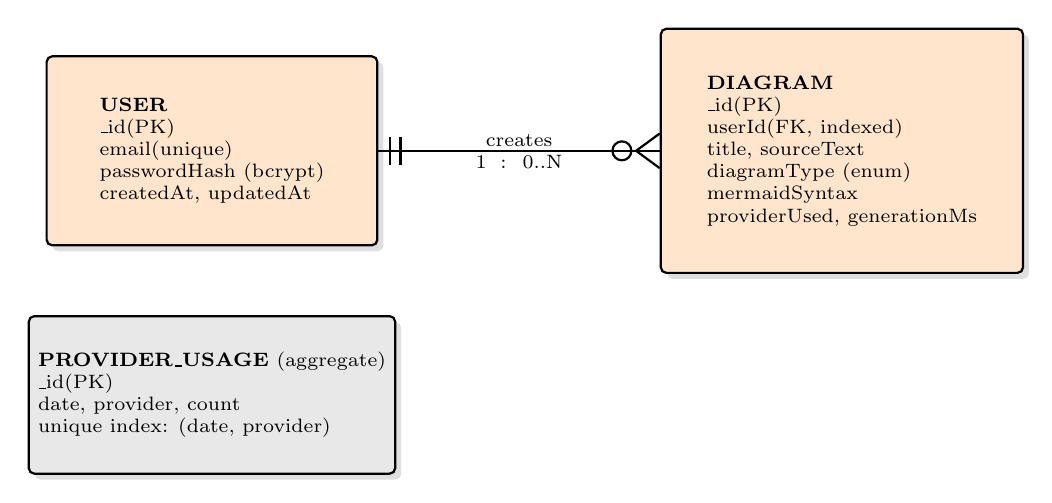
\begin{tikzpicture}
    \node[box,fill=dataTier,minimum width=4.2cm,minimum height=2.4cm,align=left,font=\scriptsize]
        (user) at (0,0) {\textbf{USER}\\\_id(PK)\\email(unique)\\passwordHash (bcrypt)\\createdAt, updatedAt};
    \node[box,fill=dataTier,minimum width=4.6cm,minimum height=3.1cm,align=left,font=\scriptsize]
        (diagram) at (8.0,0) {\textbf{DIAGRAM}\\\_id(PK)\\userId(FK, indexed)\\title, sourceText\\diagramType (enum)\\mermaidSyntax\\providerUsed, generationMs};
    \node[box,fill=infraTier,minimum width=4.2cm,minimum height=2.0cm,align=left,font=\scriptsize]
        (usage) at (0,-3.1) {\textbf{PROVIDER\_USAGE} (aggregate)\\\_id(PK)\\date, provider, count\\unique index: (date, provider)};

    \draw[thick] (user.east) -- node[lbl,above]{creates} node[lbl,below]{1 \;:\; 0..N} (diagram.west);
    \draw[thick] ($(user.east)+(0.15,0.18)$) -- ++(0,-0.36);
    \draw[thick] ($(user.east)+(0.28,0.18)$) -- ++(0,-0.36);
    \draw[thick] ($(diagram.west)+(-0.30,0)$) -- ($(diagram.west)+(0,0.22)$);
    \draw[thick] ($(diagram.west)+(-0.30,0)$) -- ($(diagram.west)+(0,-0.22)$);
    \draw[thick] ($(diagram.west)+(-0.48,0)$) circle (0.12);
\end{tikzpicture}
\caption{Entity--relationship model (crow's-foot notation, logical model enforced by Mongoose)}
\label{fig:er}
\end{figure}

\noindent The compound index \texttt{\{userId: 1, createdAt: -1\}} on
\texttt{DIAGRAM} exists because MongoDB can use a compound index only on a
\emph{prefix} of its fields. Every list query filters by \texttt{userId}
and then sorts by \texttt{createdAt}, so \texttt{userId} must come first;
reversed, the index would be useless for the most common query in the
system.

% =============================================================================
\section{Application Behaviour}
\label{sec:app-design}
% =============================================================================

\subsection{Use Case Diagram}
In Figure~\ref{fig:usecase}, \texttt{«include»} means the base use case
\emph{always} performs the included one --- generating, viewing, and
manually editing all necessarily render. \texttt{«extend»} means the
extension happens \emph{conditionally}: failover extends generation only
when the primary provider actually fails.

\begin{figure}[H]
\centering
\begin{tikzpicture}
    \node[actor,fill=clientTier] (guest) at (-5.8, 2.75) {Guest};
    \node[actor,fill=clientTier] (ruser) at (-5.8,-1.3)  {Registered\\User};
    \node[actor,fill=extTier,minimum width=2.4cm] (llm) at (7.0, 0.5) {LLM Provider\\«system»};

    \node[uc,fill=appTier]   (reg)    at (-1.4, 3.2) {Register account};
    \node[uc,fill=appTier]   (login)  at (-1.4, 2.3) {Log in};
    \node[uc,fill=secGate]   (gen)    at (-1.4, 1.2) {Generate diagram from text};
    \node[uc,fill=appTier]   (save)   at (-1.4, 0.2) {Save diagram};
    \node[uc,fill=appTier]   (view)   at (-1.4,-0.8) {View diagram};
    \node[uc,fill=appTier]   (edit)   at (-1.4,-1.8) {Edit Mermaid syntax};
    \node[uc,fill=appTier]   (del)    at (-1.4,-2.8) {Delete diagram};
    \node[uc,fill=appTier]   (export) at (-1.4,-3.8) {Export SVG / PNG};
    \node[uc,fill=secGate]   (fail)   at ( 3.0, 2.4) {Fail over to secondary};
    \node[uc,fill=infraTier] (render) at ( 3.0,-1.3) {Render diagram};

    \begin{scope}[on background layer]
        \node[boundary,fill=appTier!10,fit=(reg)(export)(fail)(render),inner xsep=0.45cm,inner ysep=0.65cm,
            label={[anchor=north,font=\bfseries\small,inner sep=3pt]north:DiagramForge}] {};
    \end{scope}

    \draw (guest) -- (reg.west);
    \draw (guest) -- (login.west);
    \foreach \u in {gen,save,view,edit,del,export} { \draw (ruser) -- (\u.west); }

    \draw[darr] (gen.south east) -- (render.west);
    \draw[darr] (view.east) -- node[lbl,above,sloped]{«include»} (render.west);
    \draw[darr] (edit.east) -- (render.west);
    \draw[darr] (fail.west) -- node[lbl,above,sloped]{«extend»} (gen.north east);

    \draw (gen.east) -- (llm.west);
    \draw (fail.east) -- (llm);
\end{tikzpicture}
\caption{Use case diagram}
\label{fig:usecase}
\end{figure}

\subsection{Control Flow: Generation, Failover, and Cost Guard}
Figure~\ref{fig:flow} is the most operationally important flow in the
system, because it encodes the cost-control logic behind \reqid{NFR-C2}.
Three invariants hold by construction, and each was checked against the
implementation:
\begin{enumerate}[nosep]
    \item \textbf{Validation happens before any paid call}, so an oversized
        input costs nothing.
    \item \textbf{The retry can happen at most once.} The ``already
        retried?'' gate routes to \texttt{502} on the second pass, so there
        is no loop and no unbounded spend.
    \item \textbf{The daily cap is checked \emph{before} the fallback call,
        never after.} A cap enforced after the money is spent is not a cap
        --- it is a report.
\end{enumerate}

\begin{figure}[p]
\centering
\resizebox{\textwidth}{!}{%
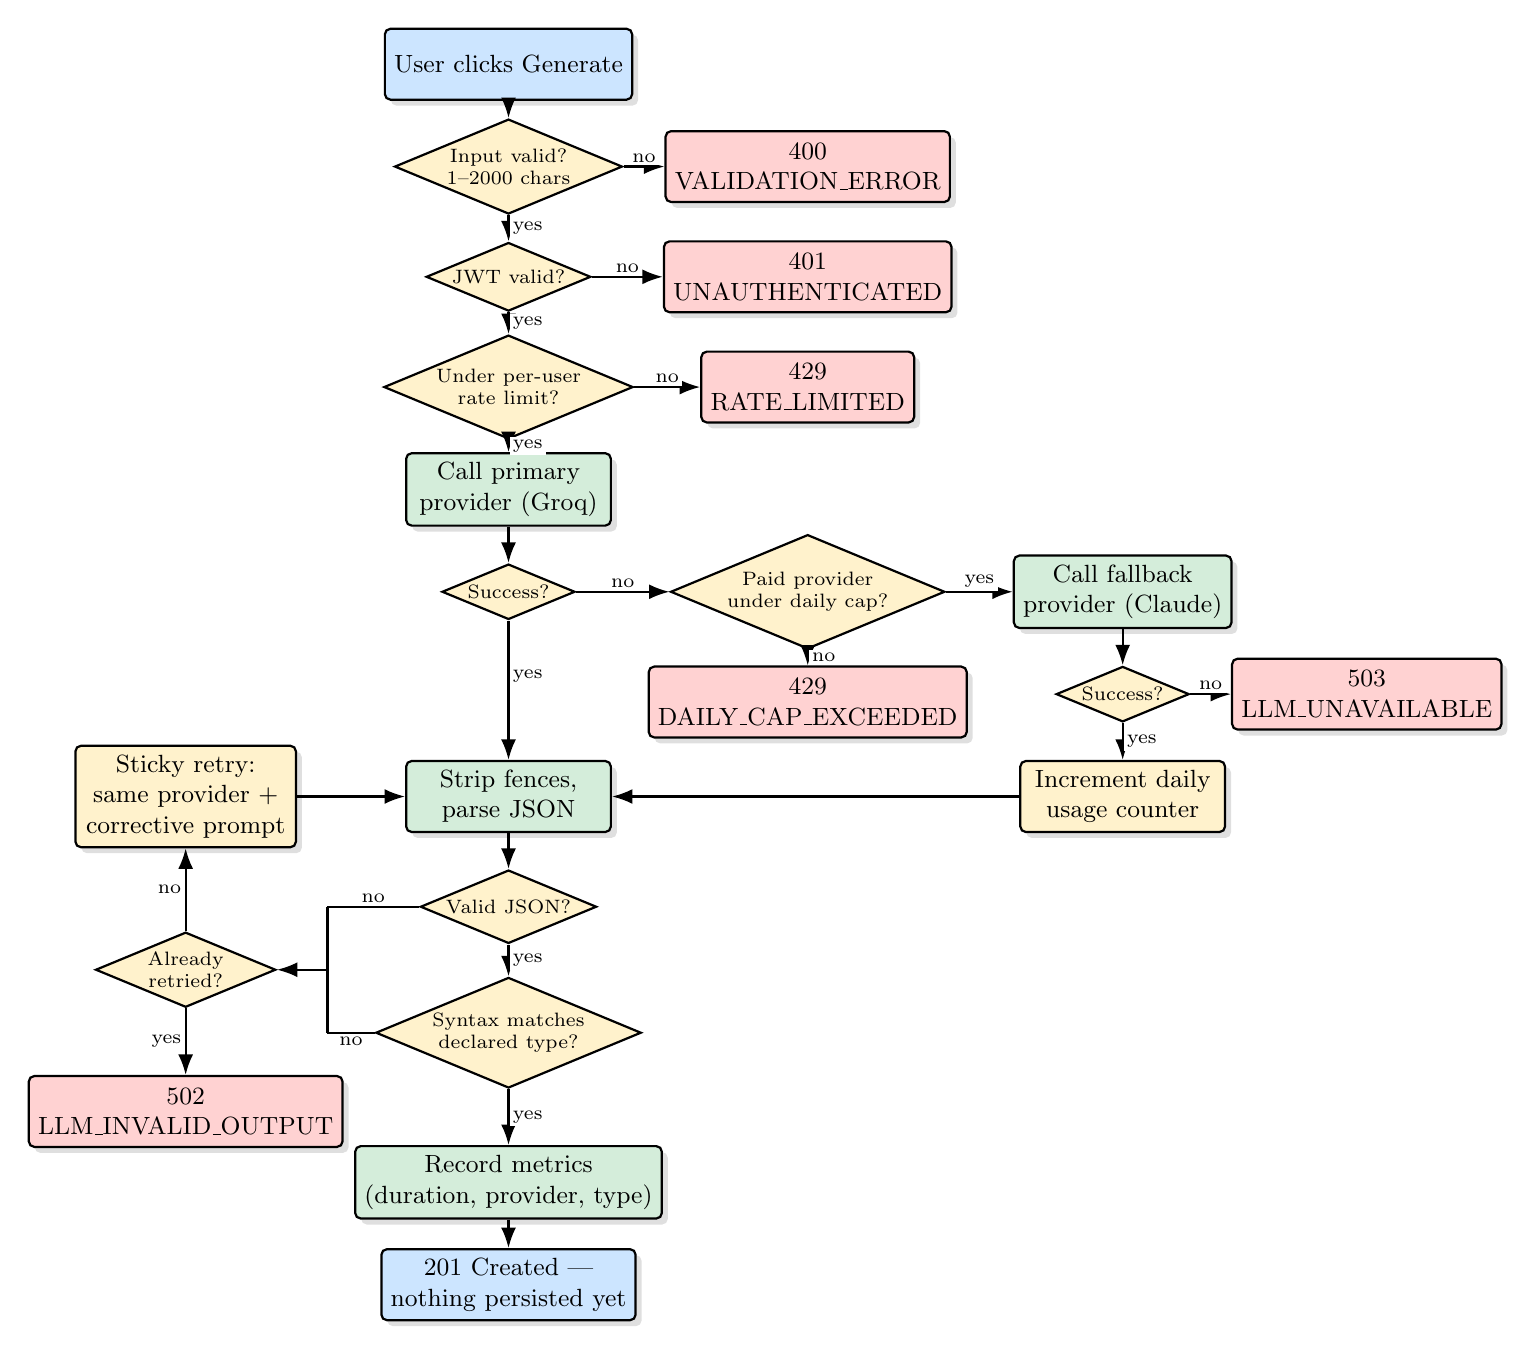
\begin{tikzpicture}[every node/.append style={font=\scriptsize}]
    % main spine
    \node[box,fill=clientTier] (start)    at (0,  0.0)  {User clicks Generate};
    \node[gate]                (valid)    at (0, -1.3)  {Input valid?\\1--2000 chars};
    \node[gate]                (auth)     at (0, -2.7)  {JWT valid?};
    \node[gate]                (rate)     at (0, -4.1)  {Under per-user\\rate limit?};
    \node[box,fill=appTier]    (primary)  at (0, -5.4)  {Call primary\\provider (Groq)};
    \node[gate]                (pok)      at (0, -6.7)  {Success?};
    \node[box,fill=appTier]    (parse)    at (0, -9.3)  {Strip fences,\\parse JSON};
    \node[gate]                (pjok)     at (0,-10.7)  {Valid JSON?};
    \node[gate]                (verify)   at (0,-12.3)  {Syntax matches\\declared type?};
    \node[box,fill=appTier]    (emit)     at (0,-14.2)  {Record metrics\\(duration, provider, type)};
    \node[box,fill=clientTier] (ret)      at (0,-15.5)  {201 Created ---\\nothing persisted yet};
    % early rejections
    \node[box,fill=ciTier]     (e400)     at (3.8,-1.3) {400\\VALIDATION\_ERROR};
    \node[box,fill=ciTier]     (e401)     at (3.8,-2.7) {401\\UNAUTHENTICATED};
    \node[box,fill=ciTier]     (e429a)    at (3.8,-4.1) {429\\RATE\_LIMITED};
    % fallback path
    \node[gate]                (cap)      at (3.8,-6.7) {Paid provider\\under daily cap?};
    \node[box,fill=ciTier]     (e429b)    at (3.8,-8.1) {429\\DAILY\_CAP\_EXCEEDED};
    \node[box,fill=appTier]    (fallback) at (7.8,-6.7) {Call fallback\\provider (Claude)};
    \node[gate]                (fok)      at (7.8,-8.0) {Success?};
    \node[box,fill=ciTier]     (e503)     at (10.9,-8.0) {503\\LLM\_UNAVAILABLE};
    \node[box,fill=secGate]    (record)   at (7.8,-9.3) {Increment daily\\usage counter};
    % retry path
    \node[box,fill=secGate,minimum width=2.8cm] (sticky) at (-4.1,-9.3) {Sticky retry:\\same provider +\\corrective prompt};
    \node[gate]                (retried)  at (-4.1,-11.5) {Already\\retried?};
    \node[box,fill=ciTier]     (e502)     at (-4.1,-13.3) {502\\LLM\_INVALID\_OUTPUT};

    \draw[arr] (start) -- (valid);
    \draw[arr] (valid) -- node[lbl,right]{yes} (auth);
    \draw[arr] (valid) -- node[lbl,above]{no} (e400);
    \draw[arr] (auth) -- node[lbl,right]{yes} (rate);
    \draw[arr] (auth) -- node[lbl,above]{no} (e401);
    \draw[arr] (rate) -- node[lbl,right]{yes} (primary);
    \draw[arr] (rate) -- node[lbl,above]{no} (e429a);
    \draw[arr] (primary) -- (pok);
    \draw[arr] (pok) -- node[lbl,right,pos=0.4]{yes} (parse);
    \draw[arr] (pok) -- node[lbl,above]{no} (cap);
    \draw[arr] (cap) -- node[lbl,right]{no} (e429b);
    \draw[arr] (cap) -- node[lbl,above]{yes} (fallback);
    \draw[arr] (fallback) -- (fok);
    \draw[arr] (fok) -- node[lbl,above]{no} (e503);
    \draw[arr] (fok) -- node[lbl,right]{yes} (record);
    \draw[arr] (record) -- (parse);

    \draw[arr] (parse) -- (pjok);
    \draw[arr] (pjok) -- node[lbl,right]{yes} (verify);
    \draw[arr] (verify) -- node[lbl,right]{yes} (emit);
    \draw[arr] (emit) -- (ret);

    % both "no" exits merge on a bus before the retry gate
    \draw[thick] (pjok.west) -- node[lbl,above]{no} (-2.3,-10.7);
    \draw[thick] (verify.west) -- node[lbl,below]{no} (-2.3,-12.3);
    \draw[thick] (-2.3,-10.7) -- (-2.3,-12.3);
    \draw[arr]   (-2.3,-11.5) -- (retried.east);
    \draw[arr]   (retried) -- node[lbl,left]{no} (sticky);
    \draw[arr]   (retried) -- node[lbl,left]{yes} (e502);
    \draw[arr]   (sticky) -- (parse);
\end{tikzpicture}}
\caption{Generation, failover, and cost-guard control flow}
\label{fig:flow}
\end{figure}

\subsection{Diagram Lifecycle}
Figure~\ref{fig:state} shows the lifecycle of a diagram from the user's
point of view. The transition worth highlighting is
\texttt{Rendered}~$\to$~\texttt{Composing}: discarding a result is a
first-class, free action, because generation never persists
(\reqid{FR-G7}) --- a bad draft leaves no orphaned row to clean up.
\texttt{SyntaxError} is likewise contained: a Mermaid parse failure renders
an inline error, and the page remains usable (\reqid{FR-D8}).

\begin{figure}[H]
\centering
\resizebox{\textwidth}{!}{%
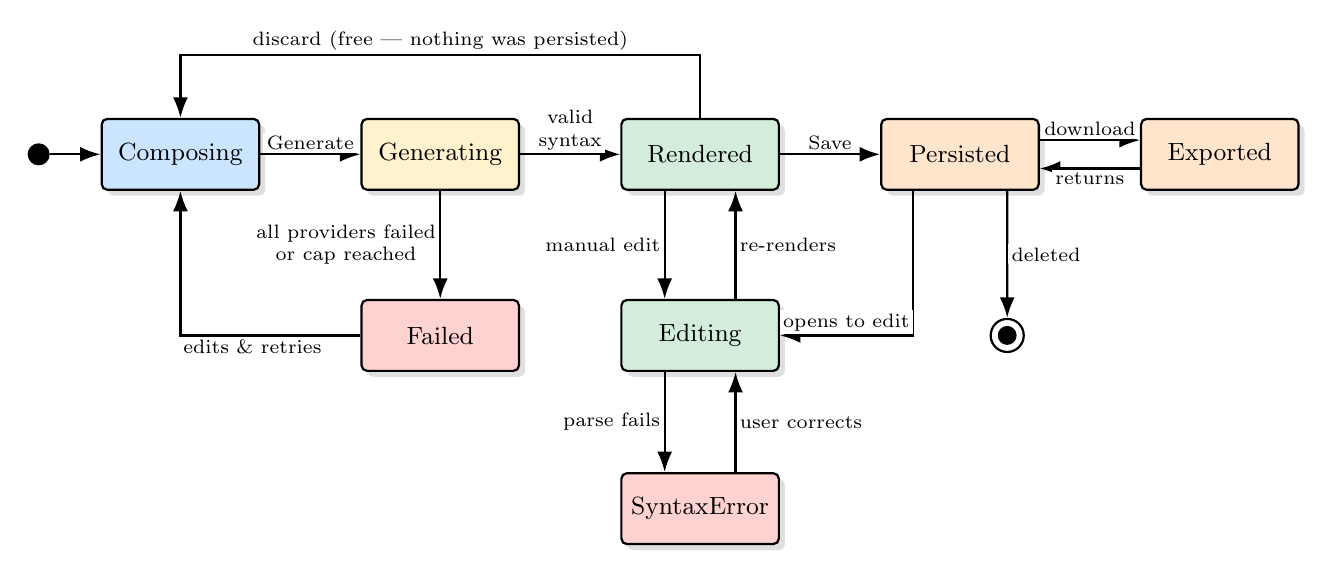
\begin{tikzpicture}[every node/.append style={font=\small}]
    \node[circle,fill=black,minimum size=0.28cm,inner sep=0] (init) at (-1.8,0) {};
    \node[box,fill=clientTier,minimum width=2.0cm] (comp)   at ( 0.0, 0.0) {Composing};
    \node[box,fill=secGate,minimum width=2.0cm]    (gen)    at ( 3.3, 0.0) {Generating};
    \node[box,fill=appTier,minimum width=2.0cm]    (rend)   at ( 6.6, 0.0) {Rendered};
    \node[box,fill=dataTier,minimum width=2.0cm]   (pers)   at ( 9.9, 0.0) {Persisted};
    \node[box,fill=dataTier,minimum width=2.0cm]   (expo)   at (13.2, 0.0) {Exported};
    \node[box,fill=ciTier,minimum width=2.0cm]     (fail)   at ( 3.3,-2.3) {Failed};
    \node[box,fill=appTier,minimum width=2.0cm]    (edit)   at ( 6.6,-2.3) {Editing};
    \node[box,fill=ciTier,minimum width=2.0cm]     (synerr) at ( 6.6,-4.5) {SyntaxError};
    \node[circle,draw,thick,minimum size=0.42cm,inner sep=0] (fin) at (10.5,-2.3) {};
    \node[circle,fill=black,minimum size=0.24cm,inner sep=0] at (fin) {};

    \draw[arr] (init) -- (comp);
    \draw[arr] (comp) -- node[lbl,above]{Generate} (gen);
    \draw[arr] (gen) -- node[lbl,above]{valid\\syntax} (rend);
    \draw[arr] (gen) -- node[lbl,left]{all providers failed\\or cap reached} (fail);
    \draw[arr] (fail.west) -| node[lbl,pos=0.3,below]{edits \& retries} (comp.south);
    \draw[arr] (rend) -- node[lbl,above]{Save} (pers);
    \draw[arr] (rend.north) -- ++(0,0.8) -| node[lbl,pos=0.25,above]{discard (free --- nothing was persisted)} (comp.north);
    \draw[arr] ($(rend.south)+(-0.45,0)$) -- node[lbl,left]{manual edit} ($(edit.north)+(-0.45,0)$);
    \draw[arr] ($(edit.north)+(0.45,0)$) -- node[lbl,right]{re-renders} ($(rend.south)+(0.45,0)$);
    \draw[arr] ($(edit.south)+(-0.45,0)$) -- node[lbl,left]{parse fails} ($(synerr.north)+(-0.45,0)$);
    \draw[arr] ($(synerr.north)+(0.45,0)$) -- node[lbl,right]{user corrects} ($(edit.south)+(0.45,0)$);
    \draw[arr] ($(pers.south)+(-0.6,0)$) |- node[lbl,pos=0.75,above]{opens to edit} (edit.east);
    \draw[arr] ($(pers.south)+(0.6,0)$) -- node[lbl,right]{deleted} (fin.north);
    \draw[arr] ($(pers.east)+(0,0.18)$) -- node[lbl,above]{download} ($(expo.west)+(0,0.18)$);
    \draw[arr] ($(expo.west)+(0,-0.18)$) -- node[lbl,below]{returns} ($(pers.east)+(0,-0.18)$);
\end{tikzpicture}}
\caption{Diagram lifecycle state diagram}
\label{fig:state}
\end{figure}

% =============================================================================
\section{DevSecOps Pipeline and Infrastructure}
\label{sec:devsecops}
% =============================================================================

This section is the operational centre of the project: every piece of
infrastructure is provisioned as code, and every code change passes an
automated, security-gated pipeline before it can reach a running
environment.

\subsection{Infrastructure as Code}
All AWS infrastructure --- VPC, security groups, IAM roles, the Jenkins EC2
instance, the EKS cluster and its node groups, and the ECR repositories ---
is defined in Terraform modules under \texttt{infrastructure/}. State is
stored remotely in S3 and locked through DynamoDB, so it is safe to share
and cannot be corrupted by two concurrent applies. Two deliberate
cost/security trade-offs are recorded here rather than hidden:
\begin{itemize}[nosep]
    \item \textbf{Worker nodes sit in public subnets}, avoiding a NAT
        Gateway (about \$32/month plus data charges). This is a real
        security trade-off, made for cost and called out explicitly.
    \item \textbf{MongoDB runs as a single-replica StatefulSet}, not a
        replica set --- an honest limitation, recorded for the
        production-readiness review in Phase~16.
\end{itemize}

\subsection{CI/CD Pipeline Architecture}
The pipeline runs on Jenkins as a Multibranch Pipeline job per service. Each
DevSecOps gate is implemented once, as a reusable step in a
\textbf{Jenkins Shared Library} --- \texttt{sonarQubeScan()},
\texttt{owaspDependencyCheck()}, \texttt{trivyScan()}, and
\texttt{pushToECR()} --- kept in its own Git repository, because Jenkins
can only load a shared library from the root of a repository.
Figure~\ref{fig:cicd} shows the backend pipeline; the frontend pipeline is
identical apart from the unit-test stage. Any gate can fail the build
independently, a failure skips every later stage, and workspace cleanup
(\texttt{cleanWs()}) always runs.

\begin{figure}[H]
\centering
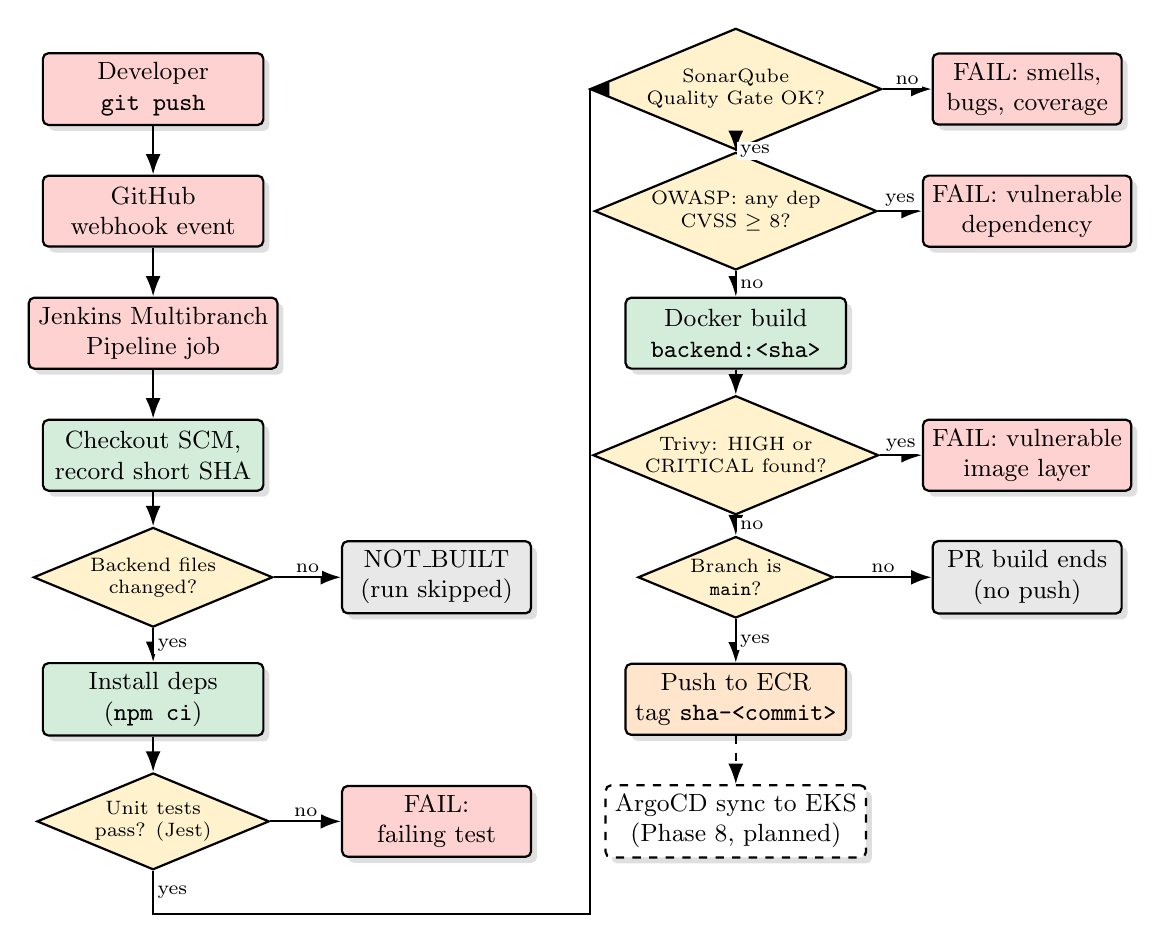
\begin{tikzpicture}[every node/.append style={font=\scriptsize}]
    % left column: trigger and build preparation
    \node[box,fill=ciTier,minimum width=2.8cm]    (push) at (0, 0.00) {Developer\\\texttt{git push}};
    \node[box,fill=ciTier,minimum width=2.8cm]    (gh)   at (0,-1.55) {GitHub\\webhook event};
    \node[box,fill=ciTier,minimum width=2.8cm]    (job)  at (0,-3.10) {Jenkins Multibranch\\Pipeline job};
    \node[box,fill=appTier,minimum width=2.8cm]   (co)   at (0,-4.65) {Checkout SCM,\\record short SHA};
    \node[gate]                                    (rel)  at (0,-6.20) {Backend files\\changed?};
    \node[box,fill=appTier,minimum width=2.8cm]   (inst) at (0,-7.75) {Install deps\\(\texttt{npm ci})};
    \node[gate]                                    (unit) at (0,-9.30) {Unit tests\\pass? (Jest)};
    \node[box,fill=infraTier,minimum width=2.4cm] (skip) at (3.6,-6.20) {NOT\_BUILT\\(run skipped)};
    \node[box,fill=ciTier,minimum width=2.4cm]    (funit) at (3.6,-9.30) {FAIL:\\failing test};

    % right column: security gates and delivery
    \node[gate]                                    (sq)   at (7.4, 0.00) {SonarQube\\Quality Gate OK?};
    \node[gate]                                    (ow)   at (7.4,-1.55) {OWASP: any dep\\CVSS $\geq$ 8?};
    \node[box,fill=appTier,minimum width=2.8cm]   (dock) at (7.4,-3.10) {Docker build\\\texttt{backend:<sha>}};
    \node[gate]                                    (tv)   at (7.4,-4.65) {Trivy: HIGH or\\CRITICAL found?};
    \node[gate]                                    (mb)   at (7.4,-6.20) {Branch is\\\texttt{main}?};
    \node[box,fill=dataTier,minimum width=2.8cm]  (ecr)  at (7.4,-7.75) {Push to ECR\\tag \texttt{sha-<commit>}};
    \node[box,fill=white,dashed,minimum width=2.8cm] (argo) at (7.4,-9.30) {ArgoCD sync to EKS\\(Phase 8, planned)};
    \node[box,fill=ciTier,minimum width=2.4cm]    (fsq)  at (11.1, 0.00) {FAIL: smells,\\bugs, coverage};
    \node[box,fill=ciTier,minimum width=2.4cm]    (fow)  at (11.1,-1.55) {FAIL: vulnerable\\dependency};
    \node[box,fill=ciTier,minimum width=2.4cm]    (ftv)  at (11.1,-4.65) {FAIL: vulnerable\\image layer};
    \node[box,fill=infraTier,minimum width=2.4cm] (nop)  at (11.1,-6.20) {PR build ends\\(no push)};

    \draw[arr] (push) -- (gh);
    \draw[arr] (gh) -- (job);
    \draw[arr] (job) -- (co);
    \draw[arr] (co) -- (rel);
    \draw[arr] (rel) -- node[lbl,right]{yes} (inst);
    \draw[arr] (rel) -- node[lbl,above]{no} (skip);
    \draw[arr] (inst) -- (unit);
    \draw[arr] (unit) -- node[lbl,above]{no} (funit);
    \draw[arr] (unit.south) -- node[lbl,right]{yes} ++(0,-0.55) -| (5.55,0) -- (sq.west);

    \draw[arr] (sq) -- node[lbl,above]{no} (fsq);
    \draw[arr] (sq) -- node[lbl,right]{yes} (ow);
    \draw[arr] (ow) -- node[lbl,above]{yes} (fow);
    \draw[arr] (ow) -- node[lbl,right]{no} (dock);
    \draw[arr] (dock) -- (tv);
    \draw[arr] (tv) -- node[lbl,above]{yes} (ftv);
    \draw[arr] (tv) -- node[lbl,right]{no} (mb);
    \draw[arr] (mb) -- node[lbl,above]{no} (nop);
    \draw[arr] (mb) -- node[lbl,right]{yes} (ecr);
    \draw[darr] (ecr) -- (argo);
\end{tikzpicture}
\caption{CI/CD pipeline with DevSecOps gates (backend service)}
\label{fig:cicd}
\end{figure}

\subsection{Security Gates in Detail}
Table~\ref{tab:gates} summarises each gate, the tool behind it, and the
requirement it enforces.

\begin{table}[H]
\centering
\begin{tabularx}{\textwidth}{@{}L{2.6cm} L{4.4cm} Y@{}}
\toprule
\textbf{Gate} & \textbf{Tool and configuration} & \textbf{What it enforces} \\
\midrule
Static analysis &
    SonarQube, via the \texttt{withSonarQubeEnv} and
    \texttt{waitForQualityGate} pipeline steps &
    Bugs, code smells, security hotspots, and coverage thresholds on
    \emph{new} code. The quality-gate result is delivered back to Jenkins
    by a SonarQube webhook. \\
Software composition analysis &
    OWASP Dependency-Check, \texttt{-{}-failOnCVSS 8}, with a persistent
    local NVD cache &
    \reqid{NFR-S5}: the build fails if any dependency carries a known CVE
    with CVSS $\geq$ 8. \\
Container image scanning &
    Trivy, \texttt{-{}-severity HIGH,CRITICAL -{}-exit-code 1} &
    \reqid{NFR-S5} (image half): the build fails if the built image
    contains a HIGH or CRITICAL vulnerability, at either the OS-package
    layer or the language-ecosystem layer. \\
Registry push &
    Amazon ECR, immutable tags, tag \texttt{sha-<commit>} &
    Runs only on \texttt{main}, and only after every earlier gate has
    passed. Tagging by Git SHA keeps every running image traceable to the
    exact source that produced it. \\
\bottomrule
\end{tabularx}
\caption{DevSecOps gates and what each one enforces}
\label{tab:gates}
\end{table}

\subsubsection{Case Study: A False-Positive CVE from a CPE Vendor Collision}
While hardening the OWASP gate, a finding --- \texttt{CVE-2026-9753}, CVSS
v3 base score 8.1 --- was reported against the \texttt{mongodb} npm driver
(version 6.20.0, pulled in transitively by Mongoose). Reading the
vulnerability's own affected-software CPE ranges in the raw JSON report,
rather than the one-line summary, showed that the CVE actually describes a
\emph{MongoDB Server} aggregation-pipeline crash
(\texttt{\$\_internalApplyOplogUpdate}), fixed in \texttt{mongod} versions
7.0.35, 8.0.24, 8.2.10, and 8.3.3 --- different software with an unrelated
versioning scheme. NVD's CPE dictionary uses the same vendor/product
identifier (\texttt{cpe:2.3:a:mongodb:mongodb}) for both the server and
the driver, so CPE-based matching flags any project that merely
\emph{talks to} a MongoDB server. Upgrading the driver could never clear
the finding; this was confirmed directly, since version 6.21.0 was still
flagged. The remediation applied is a suppression rule scoped narrowly to
\texttt{pkg:npm/mongodb@*} and this single CVE ID, with its justification
recorded in the suppression file itself --- not a blanket suppression, and
not a disabled gate.

\subsubsection{Case Study: A Real Dependency Vulnerability}
The same investigation surfaced a genuine finding:
\texttt{GHSA-2883-xcg3-v3hh} in \texttt{js-yaml} 4.3.1 (pulled in by ESLint),
a CPU-exhaustion denial of service triggered by YAML merge keys, fixed in
4.3.2. This one was fixed properly, with an npm \texttt{overrides} entry
scoped to the ESLint dependency chain only, leaving an unrelated
\texttt{js-yaml} 3.x used by Jest untouched. The two cases illustrate the
distinction the gate is designed to force: a finding is either
\emph{fixed} or \emph{proven not to apply}, and the proof is written down.

\subsubsection{Case Study: An Unused \texttt{npm} CLI as Image Attack Surface}
Trivy separately reported four HIGH-severity vulnerabilities in the built
backend image, all under \texttt{usr/local/lib/node\_modules/npm/} --- that
is, inside the \texttt{npm} CLI bundled with the \texttt{node:24-alpine}
base image, not in the application's own dependencies, which showed zero
findings. The container's entrypoint invokes \texttt{node} directly and
never calls \texttt{npm} or \texttt{npx} at runtime, so npm was only ever
needed for the image's \texttt{npm ci} build step. The fix removes npm from
the final image layer once installation completes, which eliminates the
unused attack surface rather than merely suppressing the scanner --- a
stronger remediation, available precisely because the tool was genuinely
unnecessary at runtime. It was verified by rebuilding the image, confirming
the application still starts and serves \texttt{/healthz} with HTTP~200,
and re-running Trivy to confirm zero findings.

\subsection{Deployment Architecture}
Figure~\ref{fig:deploy} shows where each component physically runs once
deployment is complete. The Jenkins server, EKS cluster, and ECR
repositories exist today; the in-cluster workloads and the ALB routing
arrive with Phases~7--8. A deliberate operational habit accompanies this
architecture: the EKS cluster and its load
balancer are torn down with \texttt{terraform destroy} at the end of each
working session and rebuilt in roughly fifteen minutes at the start of the
next, because the EKS control plane bills \$0.10/hour whether or not any
workload is running. Pods pull their images from ECR; the frontend's pull
edge is omitted from the figure for readability.

\begin{figure}[H]
\centering
\resizebox{\textwidth}{!}{%
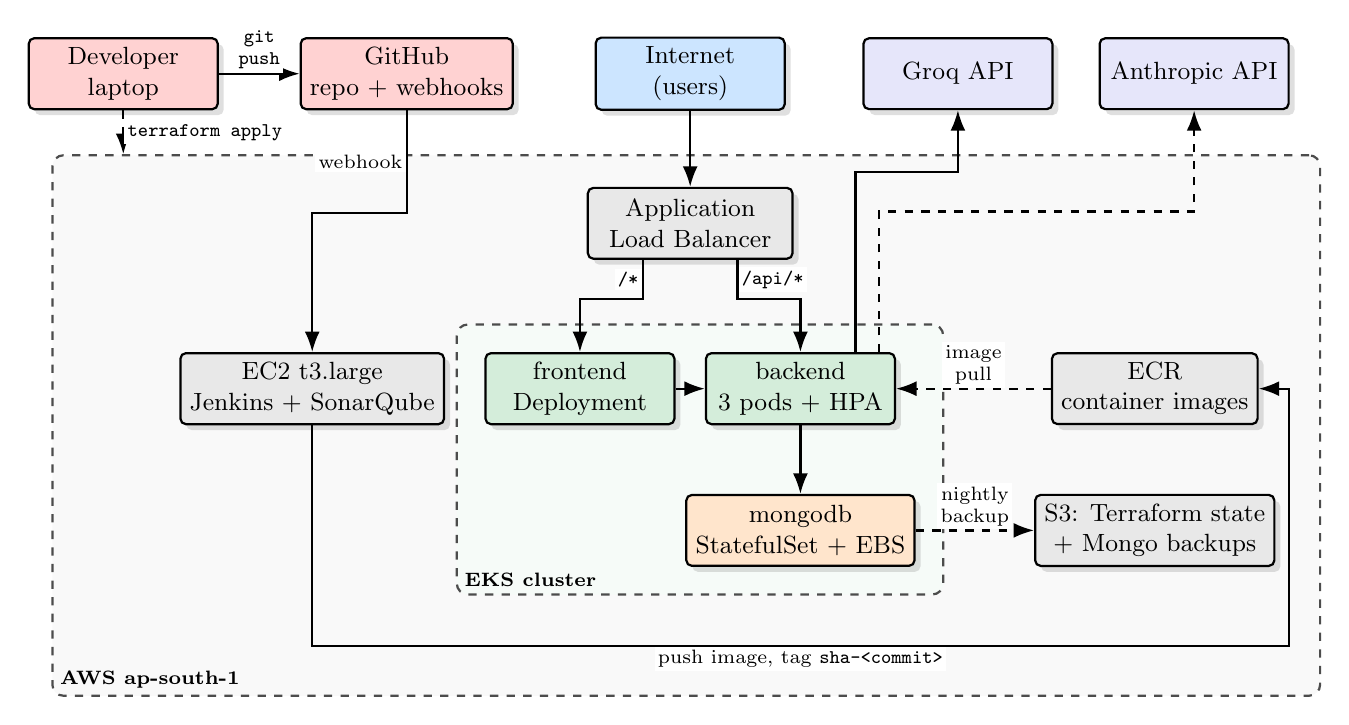
\begin{tikzpicture}[every node/.append style={font=\scriptsize}]
    % outside AWS
    \node[box,fill=ciTier,minimum width=2.4cm]     (dev)  at (-6.6, 5.2) {Developer\\laptop};
    \node[box,fill=ciTier,minimum width=2.4cm]     (gh)   at (-3.0, 5.2) {GitHub\\repo + webhooks};
    \node[box,fill=clientTier,minimum width=2.4cm] (inet) at ( 0.6, 5.2) {Internet\\(users)};
    \node[box,fill=extTier,minimum width=2.4cm]    (groq) at ( 4.0, 5.2) {Groq API};
    \node[box,fill=extTier,minimum width=2.4cm]    (anth) at ( 7.0, 5.2) {Anthropic API};
    % inside AWS
    \node[box,fill=infraTier,minimum width=2.6cm]  (alb)     at ( 0.6, 3.3) {Application\\Load Balancer};
    \node[box,fill=infraTier,minimum width=2.8cm]  (jenkins) at (-4.2, 1.2) {EC2 t3.large\\Jenkins + SonarQube};
    \node[box,fill=appTier,minimum width=2.4cm]    (fe)      at (-0.8, 1.2) {frontend\\Deployment};
    \node[box,fill=appTier,minimum width=2.4cm]    (be)      at ( 2.0, 1.2) {backend\\3 pods + HPA};
    \node[box,fill=dataTier,minimum width=2.4cm]   (mongo)   at ( 2.0,-0.6) {mongodb\\StatefulSet + EBS};
    \node[box,fill=infraTier,minimum width=2.4cm]  (ecr)     at ( 6.5, 1.2) {ECR\\container images};
    \node[box,fill=infraTier,minimum width=2.4cm]  (s3)      at ( 6.5,-0.6) {S3: Terraform state\\+ Mongo backups};

    \begin{scope}[on background layer]
        % AWS first, so the EKS box is drawn on top of its fill
        \node[boundary,fill=infraTier!25,fit={(alb)(jenkins)(ecr)(s3)(mongo)(-7.1,-2.3)(8.2,-2.3)},inner sep=0.4cm,
            label={[anchor=south west,font=\bfseries\scriptsize,inner sep=3pt]south west:AWS ap-south-1}] (aws) {};
        \node[boundary,fill=appTier!20,fit=(fe)(be)(mongo),inner sep=0.35cm,
            label={[anchor=south west,font=\bfseries\scriptsize,inner sep=3pt]south west:EKS cluster}] {};
    \end{scope}

    \draw[arr]  (dev) -- node[lbl,above]{\texttt{git}\\\texttt{push}} (gh);
    \draw[darr] (dev.south) -- node[lbl,right]{\texttt{terraform apply}} (dev.south |- aws.north);
    \draw[arr]  (gh.south) -- node[lbl,left]{webhook} ++(0,-1.3) -| (jenkins.north);
    \draw[arr]  (inet) -- (alb);
    \draw[arr]  ($(alb.south)+(-0.6,0)$) -- node[lbl,left]{\texttt{/*}} ++(0,-0.5) -| (fe.north);
    \draw[arr]  ($(alb.south)+( 0.6,0)$) -- node[lbl,right]{\texttt{/api/*}} ++(0,-0.5) -| (be.north);
    \draw[arr]  (fe) -- (be);
    \draw[arr]  (be) -- (mongo);
    \draw[arr]  ($(be.north)+(0.7,0)$) |- (4.0,3.95) -- (groq.south);
    \draw[darr] ($(be.north)+(1.0,0)$) |- (7.0,3.45) -- (anth.south);
    \draw[darr] (ecr) -- node[lbl,above]{image\\pull} (be);
    \draw[darr] (mongo) -- node[lbl,above]{nightly\\backup} (s3);
    \draw[arr]  (jenkins.south) -- ++(0,-2.8) -| node[lbl,pos=0.25,below]{push image, tag \texttt{sha-<commit>}} (8.2,1.2) -- (ecr.east);
\end{tikzpicture}}
\caption{Deployment architecture on AWS}
\label{fig:deploy}
\end{figure}

\begin{table}[H]
\centering
\begin{tabularx}{\textwidth}{@{}L{2.8cm} L{3.9cm} Y@{}}
\toprule
\textbf{Aspect} & \textbf{Choice} & \textbf{Reasoning} \\
\midrule
Region & \texttt{ap-south-1} (Mumbai) & Lowest latency from India; one
    region everywhere for consistency. \\
Worker nodes & Public subnets & Avoids a NAT Gateway (about \$32/month); a
    real, documented security trade-off. \\
MongoDB & Single-replica StatefulSet & Honest limitation; production would
    use a replica set or a managed document store. \\
Jenkins & Single EC2 instance, no HA & It is CI infrastructure, not the
    product: its downtime blocks deploys, not users. \\
Backend replicas & 3, HPA up to 10 & Survives losing one pod with headroom
    to spare (\reqid{NFR-A2}). \\
Secrets & Never in Git or images & Fetched at runtime from AWS Secrets
    Manager via the External Secrets Operator (planned, Phase~12). \\
\bottomrule
\end{tabularx}
\caption{Deployment design decisions}
\end{table}

% =============================================================================
\section{Implementation Status}
% =============================================================================

\subsection{Phase Roadmap}
The project is executed as incremental phases, each with one concrete
learning outcome (Table~\ref{tab:phases}). This report reflects the system
during Phase~6, with Phases~0--5 complete and verified.

\begin{table}[H]
\centering
\small
\begin{tabularx}{\textwidth}{@{}c L{3.3cm} Y@{}}
\toprule
\textbf{Phase} & \textbf{Focus} & \textbf{Main learning outcome} \\
\midrule
0--1 & Foundations, application & React, Express, MongoDB, Mermaid, JWT
    auth, multi-provider LLM with fallback, Docker Compose \\
2 & Jenkins infrastructure & Terraform modules, EC2, VPC, IAM, remote state \\
3 & Jenkins configuration & Configuration as Code, credentials, SonarQube
    toolchain \\
4 & EKS cluster & Kubernetes on AWS, node groups, IRSA, ALB controller \\
5 & ECR & Private registries, immutable tags, lifecycle policies \\
\textbf{6} & \textbf{CI gates} & \textbf{Jenkins pipelines, tests,
    SonarQube, OWASP Dependency-Check, Trivy (in progress; this report's
    primary subject)} \\
7 & Helm & Templated manifests, probes, HPA, StatefulSet \\
8 & GitOps & ArgoCD App-of-Apps, auto-sync, self-healing \\
9 & Observability & Prometheus, Grafana, application metrics, alerts \\
10 & DNS and TLS & Route53, ACM certificates, HTTPS through the ALB \\
11 & Persistence and backup & EBS CSI, S3 backups, restore testing \\
12 & Security hardening & External Secrets, NetworkPolicy, RBAC, Pod
    Security Standards \\
13 & Supply chain and policy & SBOM, image signing, admission policies, IaC
    scanning \\
14 & Progressive delivery & Argo Rollouts, canary releases, metric-based
    rollback \\
15 & Logs, traces, incidents & Loki, OpenTelemetry, runbooks, SLOs \\
16 & FinOps and resilience & Budgets, Karpenter, chaos tests, disaster
    recovery \\
\bottomrule
\end{tabularx}
\caption{Build roadmap}
\label{tab:phases}
\end{table}

\subsection{Verified Outcomes}
The following have been directly verified, not merely designed:
\begin{itemize}[nosep]
    \item 46 automated Jest tests across 8 suites (7 unit suites and one
        integration suite that runs against a real MongoDB instance), plus
        a real-browser Playwright check of the frontend.
    \item A passing SonarQube Quality Gate on the backend project, with the
        result delivered back to Jenkins by webhook.
    \item A clean OWASP Dependency-Check run (exit code 0) after the
        remediations described above, completing in under two minutes once
        analyzers irrelevant to an npm-only project (OSS Index, Maven
        Central, Yarn audit) were disabled --- previously over thirty
        minutes.
    \item A clean Trivy scan of the backend image (zero findings) after
        removing the unused npm CLI.
    \item Terraform-managed infrastructure with remote state (S3 plus
        DynamoDB locking), applied and destroyed repeatedly as part of the
        project's cost discipline.
\end{itemize}

% =============================================================================
\section{Security Considerations}
% =============================================================================
\begin{itemize}[nosep]
    \item \textbf{Secrets never enter version control.} CI secrets (GitHub
        token, SonarQube token, Anthropic API key, NVD API key) are stored
        as Jenkins credentials, injected with \texttt{withCredentials}, and
        masked in build logs. A committed \texttt{.env.example} documents
        variable \emph{names} and placeholders only.
    \item \textbf{Least-privilege file permissions.} The server-side
        secrets file is locked to \texttt{600 root:root}; a world-readable
        copy found during a routine audit was corrected as part of this
        work.
    \item \textbf{A known residual risk.} Jenkins masks credentials in
        build \emph{logs}, but a secret passed as a command-line argument
        remains visible in the OS process list to anyone with shell access
        on the build host. The NVD key is currently passed this way;
        moving it to an environment variable read by the tool is a
        recorded follow-up.
    \item \textbf{IAM permission additivity.} A resource-based policy, such
        as an ECR repository policy, can only \emph{add} permission; it
        cannot subtract what a principal's identity policy already grants.
        True exclusivity requires an explicit \texttt{Deny}.
    \item \textbf{Ownership checks return \texttt{404}, not \texttt{403}.}
        Confirming that a resource exists but is forbidden would let an
        attacker enumerate valid IDs.
    \item \textbf{Password handling.} bcrypt with a cost factor of 12;
        \texttt{User.toJSON()} strips \texttt{passwordHash} during
        serialisation, so the hash cannot leak even through a careless
        \texttt{res.json(user)}.
\end{itemize}

% =============================================================================
\section{Cost Model}
% =============================================================================
Table~\ref{tab:cost} shows monthly AWS cost in \texttt{ap-south-1}, running
continuously versus only during active working sessions.

\begin{table}[H]
\centering
\begin{tabularx}{\textwidth}{@{}Y r r@{}}
\toprule
\textbf{Resource} & \textbf{Always on} & \textbf{About 15 h/week} \\
\midrule
EKS control plane (\$0.10/h, billed even when idle) & \$73 & pro-rated \\
2 $\times$ t3.medium worker nodes & \$60 (\$18 spot) & pro-rated \\
Jenkins EC2 (t3.large) & \$60 & pro-rated \\
Application Load Balancer & \$18 + data & pro-rated \\
EBS volumes & \$5 & \$5 (persists) \\
Route53 hosted zone & \$0.50 & \$0.50 (persists) \\
ECR storage & negligible & negligible \\
\midrule
\textbf{Total} & \textbf{about \$215/month} & \textbf{about \$25--35/month} \\
\bottomrule
\end{tabularx}
\caption{AWS cost, always on versus disciplined teardown}
\label{tab:cost}
\end{table}

\noindent The affordability strategy is enforced by habit rather than
tooling: destroy the EKS cluster and stop the Jenkins instance at the end
of every session. That is only survivable because the whole cluster is
code --- rebuilding it by hand through the AWS console, repeatedly, would
be impractical. An AWS Budget alert is set at \$40 with a notification at
60\%.

% =============================================================================
\section{Related Work}
% =============================================================================
This project sits at the intersection of two established practices rather
than proposing a new technique in either. \textbf{GitOps} --- declarative
desired state in Git, continuously reconciled by an in-cluster controller
--- is the operating model popularised by tools such as ArgoCD and Flux, and
is used here to keep human operators out of the direct \texttt{kubectl}
path. \textbf{DevSecOps} --- shifting security scanning left into the CI
pipeline instead of treating it as a post-deployment audit --- is realised
through three independent, build-failing gates rather than one monolithic
check, so that every failure is attributable to a specific class of defect.
The case studies in Section~\ref{sec:devsecops} are offered as concrete,
reproducible illustrations of a failure mode that is common but rarely
documented in detail: CPE-based vulnerability matching that conflates
unrelated products sharing a vendor/product name in the NVD dictionary.

% =============================================================================
\section{Future Work}
% =============================================================================
The remaining phases (Table~\ref{tab:phases}) extend the platform toward a
production-representative posture:
\begin{itemize}[nosep]
    \item \textbf{Helm and GitOps} (Phases~7--8): templated charts delivered
        through ArgoCD's App-of-Apps pattern, removing the last manual
        deployment step.
    \item \textbf{Observability} (Phase~9): Prometheus and Grafana
        dashboards, with alerts derived from the SLOs in
        Table~\ref{tab:nfr-summary}.
    \item \textbf{TLS, backup, and hardening} (Phases~10--12): end-to-end
        HTTPS, restore-tested backups, Pod Security Standards, and
        NetworkPolicy enforcement.
    \item \textbf{Supply-chain security} (Phase~13): image signing with
        Cosign and admission-time policy with Kyverno, so the cluster
        refuses any image the pipeline did not sign --- closing the loop
        that the current gates open.
    \item \textbf{Progressive delivery and resilience} (Phases~14--16):
        canary releases with metric-based rollback, chaos testing, and
        FinOps controls.
\end{itemize}

% =============================================================================
\section{Conclusion}
% =============================================================================
DiagramForge shows that an instructive DevOps project does not need a
complex application --- it needs a complete one, wrapped in a platform that
is not simplified for the sake of the exercise. The application layer is
intentionally small; the pipeline, infrastructure, and security posture
around it are not. The case studies in Section~\ref{sec:devsecops} were all
found by running the gates against real code and reading the underlying
report data rather than trusting a summary line, and each was resolved
with a documented, individually justified fix. That discipline, more than
any single tool choice, is the real subject of this report.

% =============================================================================
\section*{References}
\addcontentsline{toc}{section}{References}
% =============================================================================
\begin{enumerate}[nosep,label={[\arabic*]}]
    \item OWASP Foundation. \emph{OWASP Dependency-Check}.
        \url{https://owasp.org/www-project-dependency-check/}
    \item Aqua Security. \emph{Trivy}. \url{https://trivy.dev/}
    \item SonarSource. \emph{SonarQube Documentation}.
        \url{https://docs.sonarsource.com/}
    \item National Institute of Standards and Technology. \emph{National
        Vulnerability Database}. \url{https://nvd.nist.gov/}
    \item HashiCorp. \emph{Terraform Documentation}.
        \url{https://developer.hashicorp.com/terraform}
    \item The Kubernetes Authors. \emph{Kubernetes Documentation}.
        \url{https://kubernetes.io/docs/}
    \item Jenkins Project. \emph{Pipeline and Shared Libraries}.
        \url{https://www.jenkins.io/doc/book/pipeline/shared-libraries/}
    \item OpenGitOps (CNCF). \emph{GitOps Principles v1.0.0}, 2021.
        \url{https://opengitops.dev/}
    \item S.~Bradner. \emph{Key words for use in RFCs to Indicate
        Requirement Levels}. RFC~2119, IETF, 1997.
\end{enumerate}

\end{document}
